\documentclass[11pt,a4paper]{article}
\usepackage{fontspec}
\usepackage{amsmath}
\usepackage{amsfonts}
\usepackage{amssymb}
\usepackage{graphicx}
\usepackage[spanish,es-nodecimaldot,es-lcroman,es-tabla,es-noshorthands]{babel}
\usepackage[left=3cm,right=2cm, bottom=4cm]{geometry}
\usepackage{subfigure}
\usepackage{longtable}
\usepackage{booktabs}
\usepackage{array}
\usepackage{color}
\usepackage[colorlinks=true,linkcolor=black,urlcolor=blue, unicode=true]{hyperref} 
\hypersetup{pdfencoding=auto}

\usepackage{tikz}
\usepackage{xstring}
\usepackage{./tikz-uml}


\newcolumntype{C}[1]{>{\centering\arraybackslash}m{#1}}

\definecolor{PUTCOLOR}{RGB}{46,74,255}
\definecolor{POSTCOLOR}{RGB}{187,136,0}
\definecolor{GETCOLOR}{RGB}{76,158,64}
\definecolor{DELETECOLOR}{RGB}{181,32,0}

\newcommand{\GET}{\colorbox{GETCOLOR}{GET}}
\newcommand{\POST}{\colorbox{POSTCOLOR}{POST}}
\newcommand{\PUT}{\colorbox{PUTCOLOR}{PUT}}
\newcommand{\DELETE}{\colorbox{DELETECOLOR}{DELETE}}

\setsansfont[Ligatures=TeX]{texgyreadventor}
\setmainfont[Ligatures=TeX]{texgyrepagella}

%*******************************************************
%                 NO MODIFICAR
\newcommand*{\FSfont}[1]{%
  \fontencoding{T1}\fontfamily{#1}\selectfont}

\newlength{\tpheight}\setlength{\tpheight}{0.9\textheight}
\newlength{\txtheight}\setlength{\txtheight}{0.9\tpheight}
\newlength{\tpwidth}\setlength{\tpwidth}{0.9\textwidth}
\newlength{\txtwidth}\setlength{\txtwidth}{0.9\tpwidth}
\newlength{\drop}
%*******************************************************

% Crea una portada con los siguientes parámetros
%
% #1 : Título 
% #2 : Subtítulo
% #3 : Subsubtítulo
% #4 : Autor(es)
% #5 : Lugar
%

\newcommand*{\portada}[5]{
\begin{titlepage}
\begingroup
\vspace*{1cm}
\drop = 0.2\txtheight
\centering
\vfill
{\Huge \scshape #1}\\[\baselineskip]
{\Large \textbf{#2}}\\[\baselineskip]
{\Large \scshape #3}\\[\baselineskip]
\vspace*{0.3cm}
{\large \textit{#4}}\\[0.5\drop]

\includegraphics[scale=0.35]{./imagenes/logoURJC.jpg}
\vspace*{1.5cm}

{\large \scshape #5, \today} \par
\begin{center}
\end{center}
\vfill\null
\endgroup
\end{titlepage}
}
 %*****************************************************
 

\newcommand{\anadirruta}{
\begin{tikzpicture}
\tikzumlset{fill state=white}
\umlstateinitial[name=initial]
\begin{umlstate}[x=0, y=-3,name=datos]{Iniciar sesión}
\end{umlstate}

\umlstatedecision[y=-5, name=permiso] 

\begin{umlstate}[x=0, y=-8,name=comprobar]{Ver perfil}
\end{umlstate}

\begin{umlstate}[y=-11,name=sesion]{Añadir ruta}
\end{umlstate}

\umlstatefinal[y=-13, name=final]

\umltrans{initial}{datos}
\umltrans{datos}{permiso}
\umltrans[arg1=correcto]{permiso}{comprobar}
\umltrans{comprobar}{sesion}
\umltrans{sesion}{final}
\umlHVHtrans[arg1=incorrecto, arm2=-4]{permiso}{final}

\end{tikzpicture}
}

\newcommand{\buscarruta}{
	\begin{tikzpicture}
	\tikzumlset{fill state=white}
	\umlstateinitial[name=initial]
	\begin{umlstate}[x=0, y=-3,name=datos]{Buscar ruta}
	\end{umlstate}
	
	\umlstatefinal[y=-5, name=final]
	
	\umltrans{initial}{datos}
	\umltrans{datos}{final}
	
	\end{tikzpicture}
}

\newcommand{\clasesbackend}{
	
\begin{tikzpicture}
	
\tikzumlset{fill state=white}
\umlclass[x=0, y=0]{User}{
}{
}

\umlclass[x=5, y=0]{Route}{
}{
}

\umlclass[x=8, y=0]{Stretch}{
}{
}

\umlclass[x=11, y=0]{Point}{
}{
}

\umlclass[x=8, y=-5]{Image}{
}{
}

\umlclass[x=3, y=-5]{Comment}{
}{
}

\umlclass[x=11, y=-5]{TypeRoute}{
}{
}


% Relaciones

\umlassoc[mult1=0..n, mult2=1]{User}{Route}

\umlassoc[mult1=0..n, mult2=1]{User}{Comment}

\umlassoc[mult1=1, mult2=0..n]{Route}{Image}

\umlassoc[mult1=0..n, mult2=1]{Route}{Comment}

\umlassoc[mult1=1, mult2=1]{Route}{TypeRoute}

\umlcompo{Route}{Stretch}

\umlcompo{Stretch}{Point}


\end{tikzpicture}

}

\newcommand{\tecnologias}{

\begin{tikzpicture}[scale=1]
\node[inner sep=0pt] (bower) at (0,0)
    {
\includegraphics[width=.2\textwidth]{imagenes/bower.png}};
\node[inner sep=0pt] (npm) at (0,-6)
    {
\includegraphics[width=.2\textwidth]{imagenes/node-npm.png}};
\node[inner sep=0pt] (angularjs) at (10,0)
    {
\includegraphics[width=.2\textwidth]{imagenes/angular.png}};
\node[inner sep=0pt] (npm) at (5,0)
    {
\includegraphics[width=.2\textwidth]{imagenes/spring.png}};
\node[inner sep=0pt] (npm) at (5,-6)
    {
\includegraphics[width=.2\textwidth]{imagenes/aws.png}};
\node[inner sep=0pt] (npm) at (10,-6)
    {
\includegraphics[width=.2\textwidth]{imagenes/elastic_beanstalk.png}};

\end{tikzpicture}

}

\newcommand{\clasesfrontend}{
	
\begin{tikzpicture}
	
\tikzumlset{fill state=white}
\umlclass[x=0, y=0]{Route}{
}{
}

\umlclass[x=5, y=0]{Profile}{
}{
}

\umlclass[x=-5, y=-2]{MapCtrl}{
}{
}

\umlclass[x=0, y=-2]{MapViewCtrl}{
}{
}

\umlclass[x=5, y=-2]{EditMapCtrl}{
}{
}

\umlclass[x=-5, y=-4]{PreferencesCtrl}{
}{
}

\umlclass[x=0, y=-4]{UploadCtrl}{
}{
}

\umlclass[x=0, y=-4]{UploadCtrl}{
}{
}

\umlclass[x=5, y=-4]{Comment}{
}{
}

\umlclass[x=-5, y=-6]{Login}{
}{
}

\umlclass[x=0, y=-6]{LoginCtrl}{
}{
}

\umlclass[x=5, y=-6]{ViewPublicCtrl}{
}{
}

\umlclass[x=-5, y=-8]{Register}{
}{
}

\umlclass[x=0, y=-8]{RegisterCtrl}{
}{
}

\umlclass[x=3, y=-8]{Search}{
}{
}

\umlclass[x=7, y=-8]{SearchByCategory}{
}{
}

\umlclass[x=-5, y=-10]{HomeCtrl}{
}{
}

\umlclass[x=0, y=-10]{NavCtrl}{
}{
}


% Relaciones

\umlassoc{MapCtrl}{Route}

\umlassoc{Route}{EditMapCtrl}

\umlassoc{Route}{MapViewCtrl}

\umlassoc{Comment}{MapViewCtrl}

\umlassoc{PreferencesCtrl}{UploadCtrl}

\umlassoc{Comment}{ViewPublicCtrl}

\umlassoc{Route}{MapViewCtrl}

\umlassoc{Login}{LoginCtrl}

\umlassoc{Register}{RegisterCtrl}

\umlassoc{Search}{SearchByCategory}




\end{tikzpicture}

}


\newcommand*{\autores}{
\begin{tabular}{r l}
GII+GIS: & Germán Alonso Azcutia \\
GIS:		 & Carlos Vázquez Sánchez \\
GIS+MAT: & José Ignacio Escribano Pablos
\end{tabular}
}

\begin{document}

\pagenumbering{alph}
\setcounter{page}{1}

\portada{Práctica 3}{Diseño de Aplicaciones Web}{Diseño e implementación de una  aplicación web \\ de rutas en AngularJS y Spring MVC}{\autores}{Móstoles}

\tableofcontents
\thispagestyle{empty}
\newpage

\listoffigures
\thispagestyle{empty}
\newpage

\pagenumbering{arabic}
\setcounter{page}{1}

\section{Introducción}

Para esta práctica hemos decidido diseñar e implementar una aplicación que permita a sus usuarios ver, añadir, y modificar rutas de distintos tipos como senderismo, a caballo, a vela, etc. La aplicación es similar a la existente Wikiloc, con la diferencia que nuestras rutas se crearán siempre dibujándolas mediante \textit{google maps}.

\subsection{Tecnologías empleadas}
\begin{itemize}
\item Tal y como se pedía en el enunciado  de la práctica, nuestra aplicación sigue una arquitectura SPA que utiliza Angular JS para el front-end y Spring MVC para el back end.
\item Para instlar las dependencias necesarias para el front-end hemos usado Bower.
\item Para realizar todo lo relacionado con mapas hemos usado la API de \textit{Google Maps}.
\item Angular material ha sido el framework elegido para realizar la interfaz de usuario.
\item La aplicación ha sido desplegada mediante Amazon Web Services.

\end{itemize}

\begin{figure}[htbp]
\centering
\tecnologias
\caption{Tecnologías usadas}
\label{fig:tecnologias}
\end{figure}

\clearpage

\subsection{Arquitectura del sistema}

\begin{figure}[htbp]
\centering
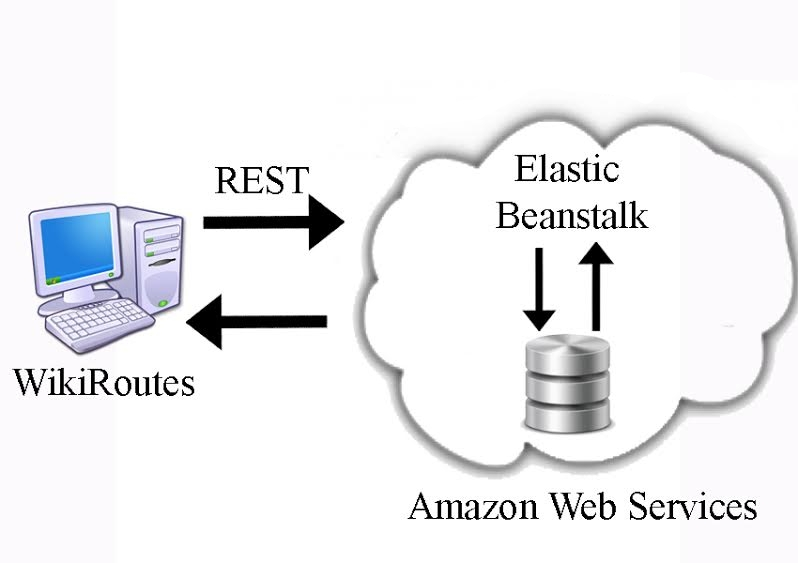
\includegraphics[width=0.7\linewidth]{imagenes/arquitectura}
\caption{Arquitectura de la aplicación}
\label{fig:arquitectura}
\end{figure}


\clearpage

\section{Diagramas UML}

A continuación, representamos los diagramas UML tanto del backend como del frontend. En el primero, de ellos, presentamos el diagrama de clases y dos diagramas de actividad; en el segundo, presentamos el diagrama de clases.

\subsection{Diagramas UML del backend}

El diagrama de clases del backend se basan en nuestra implementación de la API REST. También incluimos dos diagramas de actividades: añadir ruta y buscar ruta.  

\subsubsection{Diagrama de clases}

El diagrama de clases se compone de las clases de la API REST, entre las que se encuentran Route, Stretch, Point, User, Image, etc. (Figura \ref{fig:clases_backend})

\begin{figure}
\centering
\clasesbackend
\caption{Diagrama de clases del backend}
\label{fig:clases_backend}
\end{figure}

\subsection{Diagramas de actividad}

Los diagramas de actividad que incluimos son algunos de los más utilizados dentro de nuestra aplicación: buscar ruta y añadir ruta. No hemos querido añadir más diagramas para no hacer más extensa esta memoria.


\subsubsection{Diagrama de actividad de añadir ruta}

El diagrama de actividad de añadir ruta, indica los pasos que son reuqeridos para añadir una ruta en nuestra aplicación. Lo primero de ello es iniciar sesión, en caso de tener un usuario y contraseña válida, nos lleva a nuestro perfil para finalmente rellenar los datos de nuestra ruta. El diagrama se puede ver en la Figura \ref{fig:anadirruta}

\begin{figure}[htbp]
\centering
\anadirruta
\caption{Diagrama de actividad de añadir ruta}
\label{fig:anadirruta}
\end{figure}


\subsubsection{Diagrama de actividad de buscar ruta}

El diagrama de actividad de ruta es muy sencillo, puesto que sólo es necesario ingresar el nombre de la ruta que deseemos buscar para encontrar la ruta que busquemos. La Figura \ref{fig:buscarruta} muestra este diagrama de actividad.  

\begin{figure}
\centering
\buscarruta
\caption{Diagrama de actividad de buscar ruta}
\label{fig:buscarruta}
\end{figure}

\subsection{Diagramas UML del frontend}

En esta sección sólo incluimos los diagramas de clases, puesto que los diagramas de actividad son análogos a los anteriores.

\subsubsection{Diagrama de clases}

El diagrama de clases se corresponde con los servicios y controladores que hemos utilizado en el lado del cliente, implementado en AngularJS.\\

Se incluyen clases como Route, Comment, User, Register, etc. que son necesarias para el correcto funcionamiento de la aplicación. La Figura \ref{fig:clasesfrontend} muestra el diagrama de clases completo.

\begin{figure}
\centering
\clasesfrontend
\caption{Diagrama de clases del frontend}
\label{fig:clasesfrontend}
\end{figure}


\clearpage

\section{Recorrido por la aplicación}
\subsection{Inicio}
La primera pantalla tras iniciar la aplicación de escritorio muestra una cabecera que será común en todas las pantallas (está presente en \textit{index.html}), además de una imagen logotipo de la página y las rutas mejor valoradas. En la cabecera se podrán realizar búsquedas de rutas (se muestran posibles opciones con un autocompletado automático desplegable), filtrar resultados por categoría, un enlace a los desarrolladores y una página de ayuda. Desde esta página inicial pueden accederse al resto de las vistas de la aplicación.
\begin{figure}[h]
\centering
  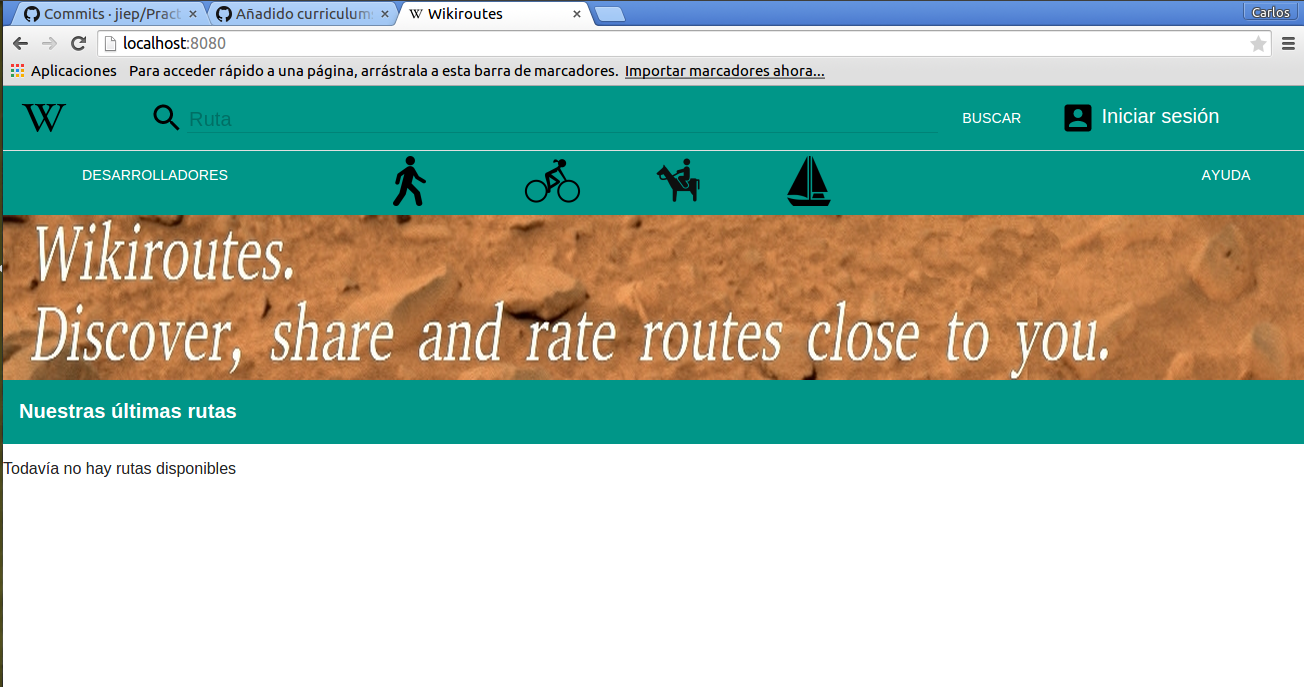
\includegraphics[width=0.7\textwidth]{./imagenes/inicial}
  \caption{Página inicial}
  \label{fig: Página inicial}
\end{figure}
\subsection{Identificación y registro}
Tras seleccionar el botón de iniciar sesión se abrirá la página desde la que un usuario puede identificarse mediante usuario y contraseña. Ambos campos son evidentemente requeridos por el sistema, por lo que si se intenta avanzar sin rellenar uno de ellos, la aplicación mostrará un pequeño diálogo indicando que campo no ha sido completado

\begin{figure}[h]
\centering
  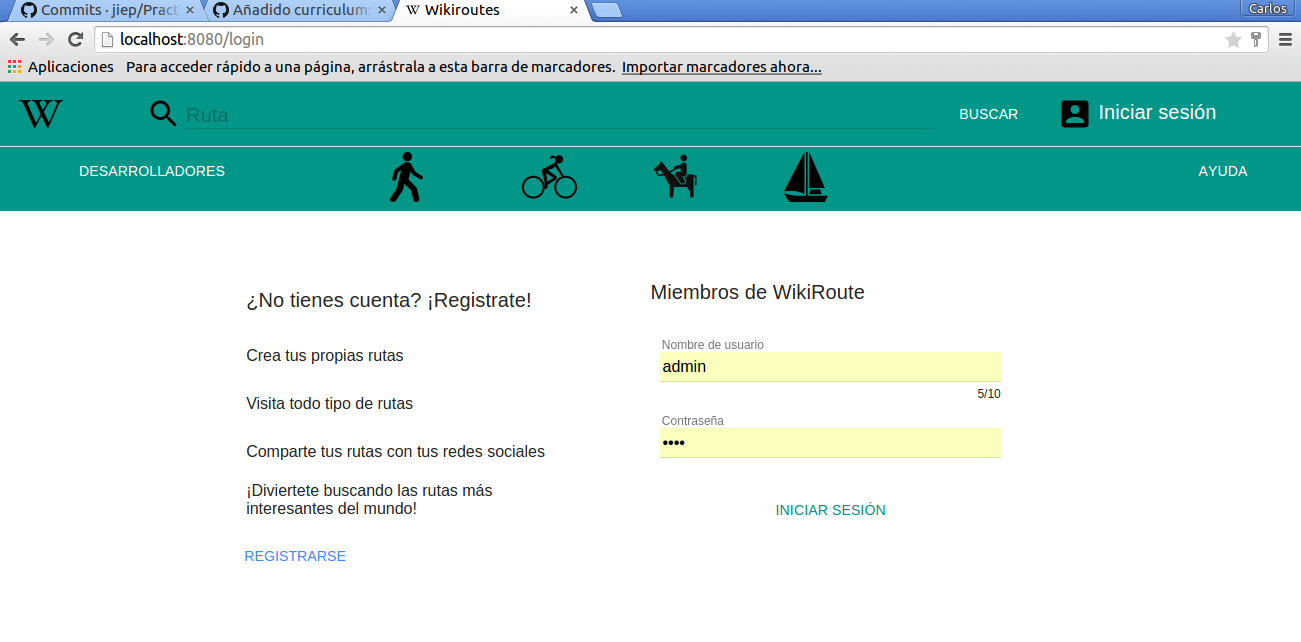
\includegraphics[width=0.7\textwidth]{./imagenes/login}
  \caption{Página de login}
  \label{fig: Página de login}
\end{figure}
En esta misma página hemos añadido también la opción para registrarse, en cuyo caso se pedirá al usuario que indique el nombre de usuario que desea (debe ser de un máximo de 10 caracteres y único), así como la contraseña, dirección de coreo electrónico y si desea recibir notificaciones por email cada vez que uno sus amigos añada una nueva ruta.\\


\begin{figure}[h]
\centering
  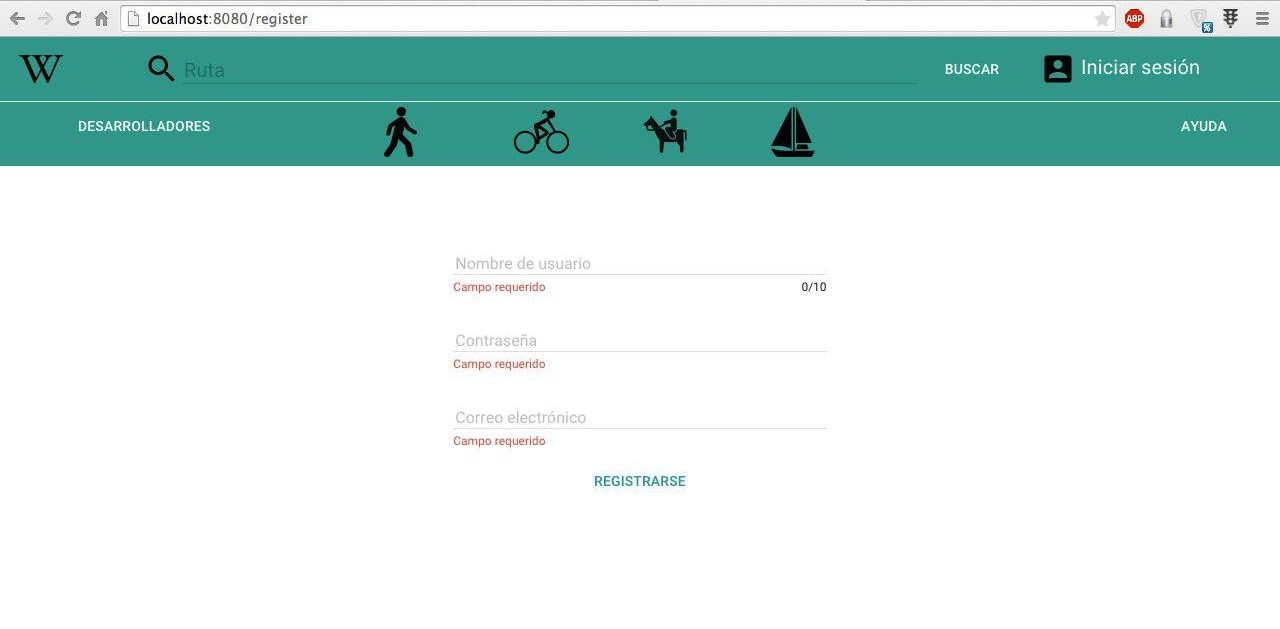
\includegraphics[width=0.7\textwidth]{./imagenes/registro}
  \caption{Página de registro}
  \label{fig: Página de registro}
\end{figure}
\clearpage
\subsection{Perfil}
Una vez registrado o autentificado correctamente, se mostrará  la página personal de cada usuario. En esta vista se mostrarán un botón para añadir una nueva ruta, así como las rutas que el usuario ha subido junto su foto, nombre, descripción y distintas opciones como editar, eliminar, hacer privada o comentar dicha ruta. 
\begin{figure}[h]
\centering
  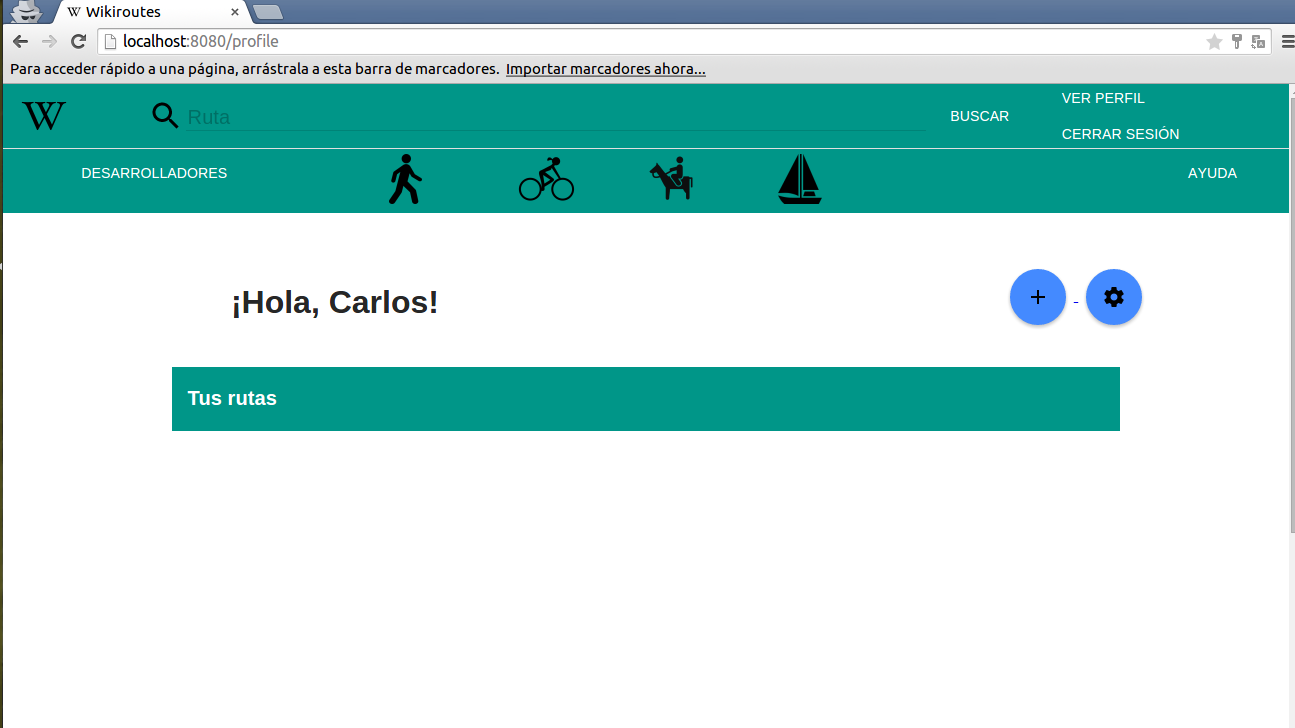
\includegraphics[width=0.7\textwidth]{./imagenes/perfil}
  \caption{Página de perfil de usuario}
  \label{fig: Página de perfil de usuario}
\end{figure}

También se dispone de una pequeña vista en la que se pueden modificar parámetros de la cuenta como correo electrónico o contraseña
\begin{figure}[h]
\centering
  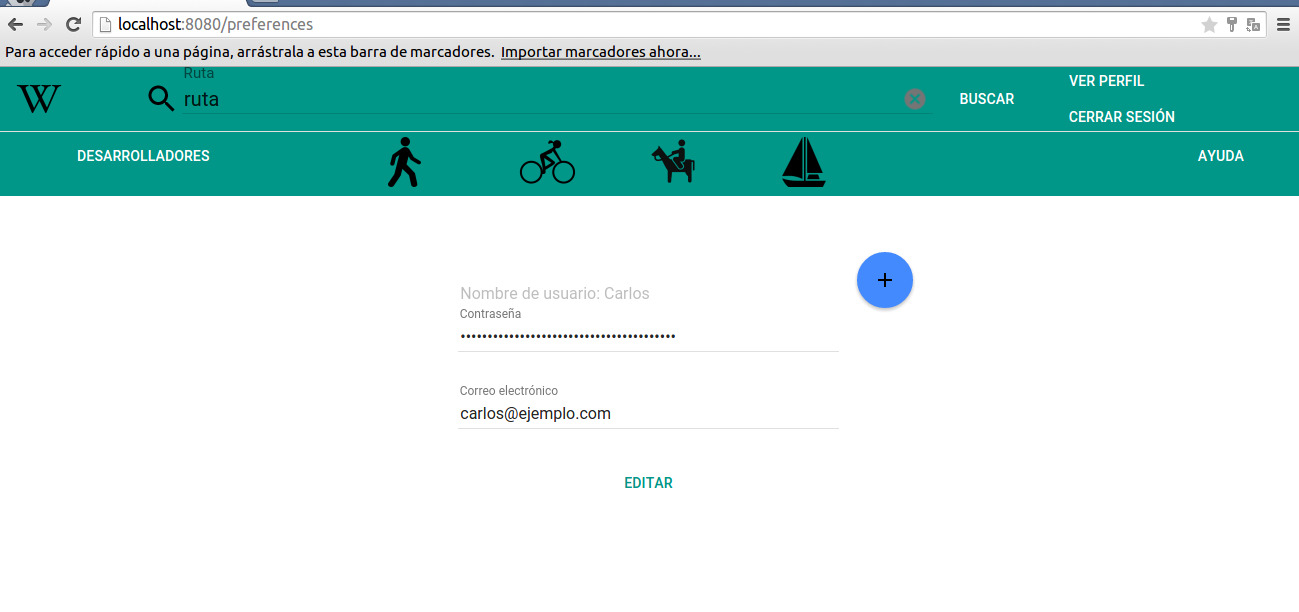
\includegraphics[width=0.7\textwidth]{./imagenes/editar}
  \caption{Página de editar perfil de usuario}
  \label{fig: Página de editar perfil de usuario}
\end{figure}
\clearpage
\subsection{Añadir y buscar rutas}
Si se selecciona el botón de añadir una nueva ruta, se mostrará la ventana más importante de nuestra aplicación: se muestra un mapa proporcionado por \textit{Google maps} sobre el que puedes crear tu ruta mediante clicks del botón izquierdo del ratón. La ruta se irá creando mediante segmentos unidos por vértices, los cuales se pueden mover a otra posición del mapa pulsando y arrastrándolos. Por suspuesto las opciones típicas de Google maps como cambiar entre las vistas de mapa/satélite, hacer zoom o moverse por el mapa están disponibles.\\
También se incluyen los campos necesarios para añadir a una ruta toda la información necesaria: nombre de la ruta (obligatorio), descripción, pública o privada, tipo de ruta y la foto que la identificará (obligatoria).\\

\begin{figure}[h]
\centering
  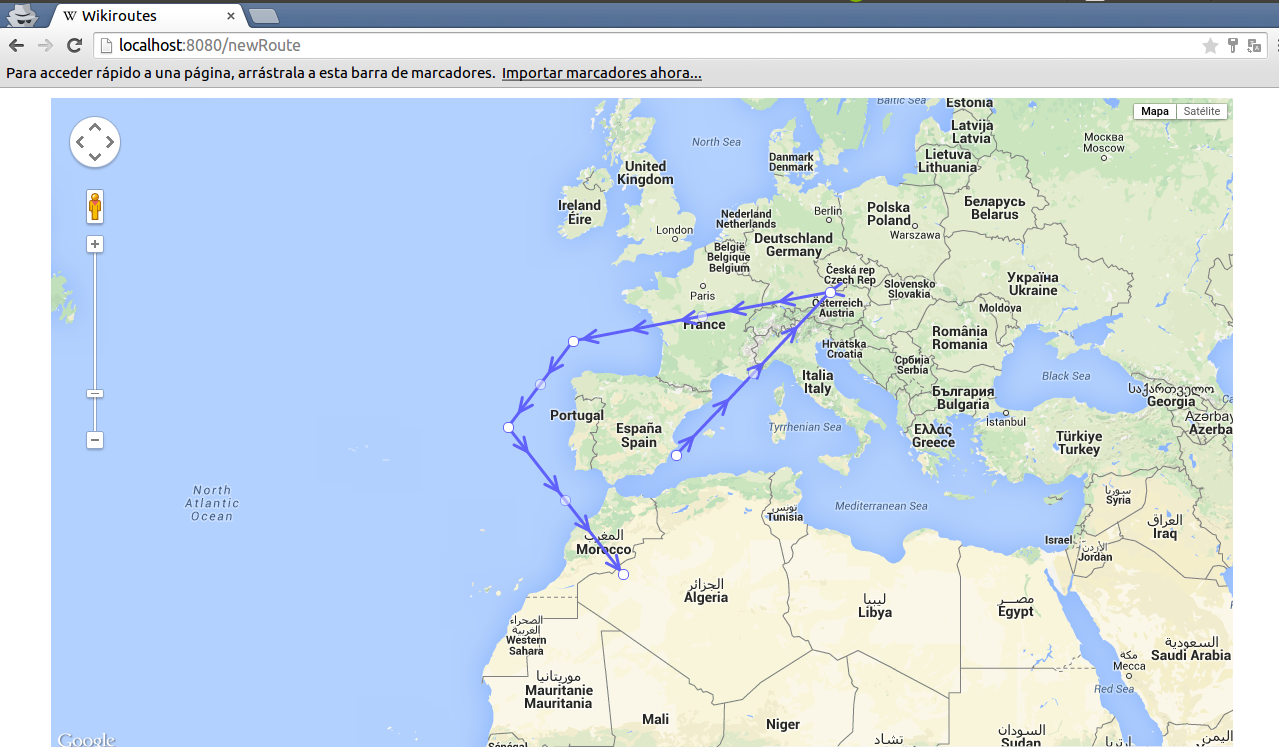
\includegraphics[width=0.7\textwidth]{./imagenes/anadir}
  \caption{Página para añadir una ruta nueva}
  \label{fig: Página para añadir una ruta nueva}
\end{figure}

Para guardar la ruta basta con completar todos los campos requeridos y pulsar el botón ``Añadir ruta'', el cual nos llevará de nuevo a nuestro perfil, dónde se puede ver nuestra ruta añadida correctamente.\\
\clearpage
\begin{figure}[h]
\centering
  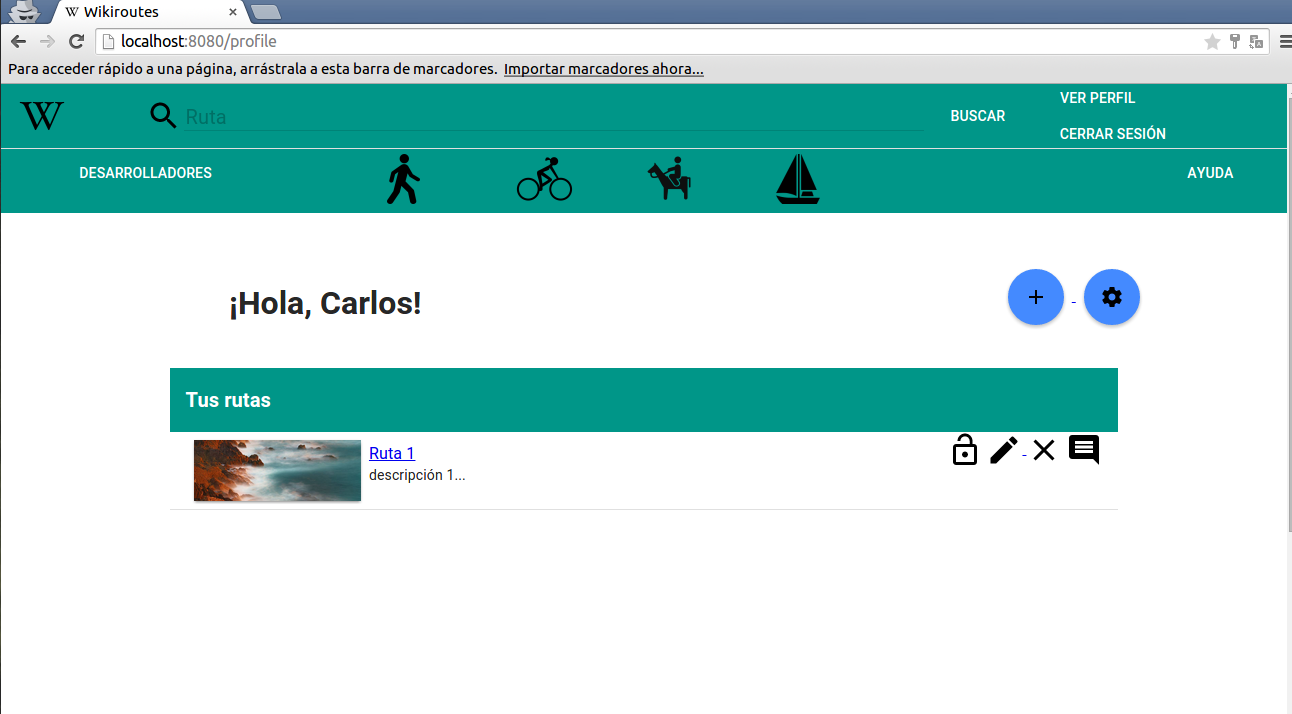
\includegraphics[width=0.7\textwidth]{./imagenes/perfilanadir}
  \caption{Página de perfil con rutas añadidas}
  \label{fig: Página de perfil con rutas añadidas}
\end{figure}

Citar que las rutas que hemos añadido pueden localizarse desde el buscador, en cuyo caso redirigirían a la vista que acabamos de explicar.\\

\begin{figure}[h]
\centering
  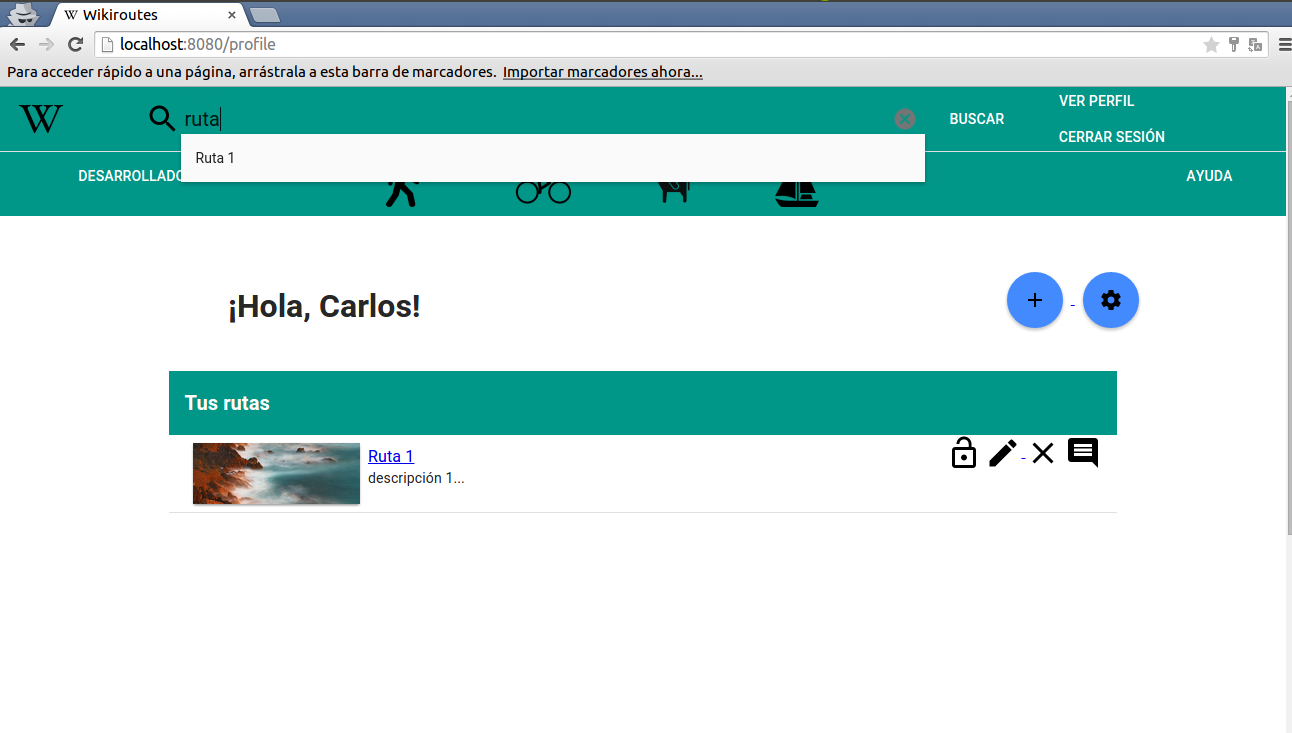
\includegraphics[width=0.7\textwidth]{./imagenes/buscar}
  \caption{Página de búsqueda de ruta}
  \label{fig: Página de búsqueda de ruta}
\end{figure}

Además pueden añadirse a comentarios siempre que la ruta se haya declarado como pública. Para ello podemos acceder a la ruta a través de la página principal, buscando por nombre, categoría o desde la página de perfil de usuario. Si se accede a la página sin identificarse, no se podrá comentar.
\begin{figure}[h]
\centering
  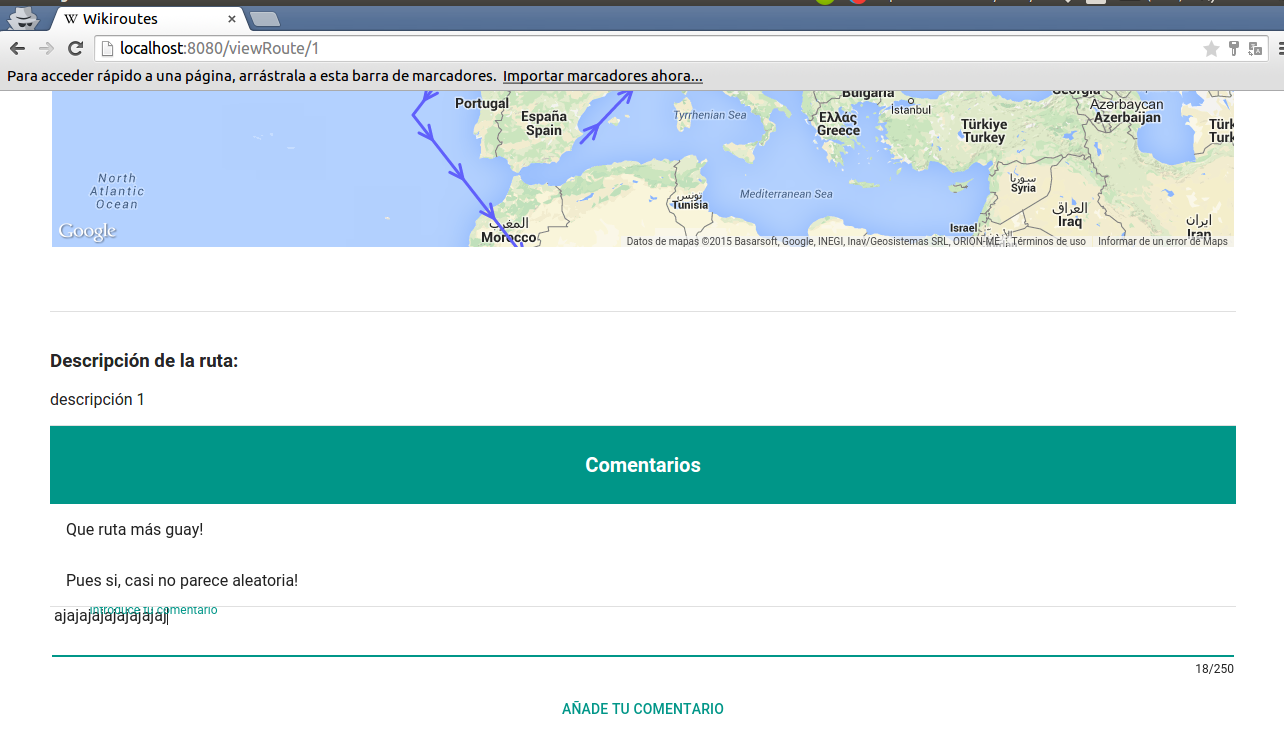
\includegraphics[width=0.7\textwidth]{./imagenes/comentarios}
  \caption{Página de comentarios de una ruta}
  \label{fig: Página de comentarios de una ruta}
\end{figure}

\subsection{Desarrolladores}
Por último hemos añadido una página de ``developers'', en la que mostramos brevemente los creadores de la página web, así como enlaces a sus linkedin, github o twitter.
\begin{figure}[h]
\centering
  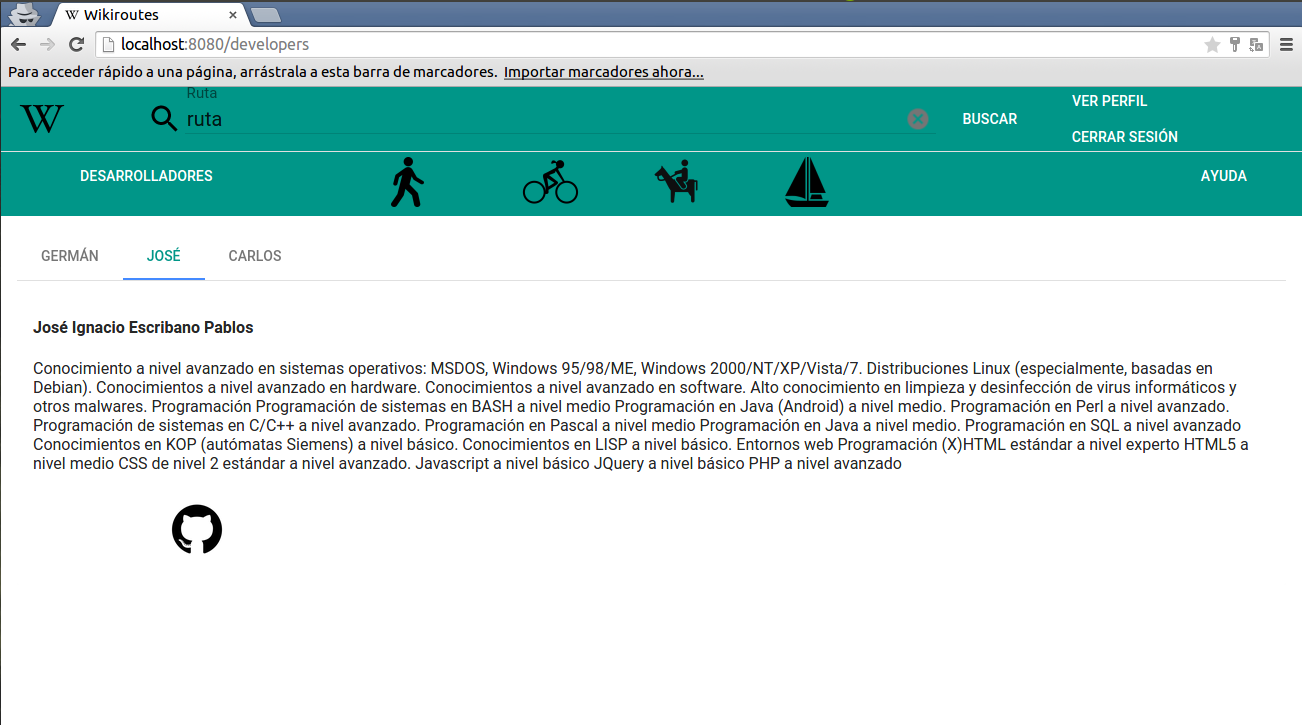
\includegraphics[width=0.7\textwidth]{./imagenes/developers}
  \caption{Página de búsqueda de ruta}
  \label{fig: Página de búsqueda de developers}
\end{figure}

\clearpage

\section{Mejoras futuras}
Ha habido numerosas funcionalidades que no hemos podido implementar por falta de tiempo. A continuación mostramos las mejoras más significativas que incorporaría una hipotética siguiente versión:
\begin{itemize}
\item La más importante: se añadiría una versión para móviles. Esta fue la principal motivación que nos llevó a desplegar la aplicación en AWS, ya que evidentemente no podíamos ejecutar nuestra aplicación fácilmente en nuestro móvil a través de \textit{localhost}. Esta aplicación tendría las vistas realizadas con el framework ionic.
\item Un sistema real de ``amigos''. Esta funcionalidad permitiría a los usuarios añadir amigos a su lista, los cuales recibirían (si lo tienen habilitado en sus preferencias) notificaciones por correo cada vez que el usuario subiera una nueva ruta. Por supuesto estarían disponibles las opciones de bloquear y denunciar usuario. Esta relación sería bidireccional, es decir, si un usuario añade a amigos a otro usuario y éste confirma la solicitud, ambos podrían ver las novedades del otro usuario, así como sus rutas privadas.
\item Mejorar el sistema de búsqueda de usuarios, de forma que en el buscador se puedan encontrar tanto rutas como usuarios.
\item Añadir más interacción con las redes sociales: se incorporaría el timeline embebido de la cuenta de twitter de la aplicación, así como los típicos botones para darle a me gusta en facebook, google+, etc.
\item Incorporar un sistema de calificación de rutas. Se realizaría mediante un sistema de puntuación de 5 estrellas, simimlar al utilizado por amazon. Esta puntuación serviría para actualizar las rutas más valoradas o filtrar los resultados según su puntuación.
\item Dar más flexibilidad al perfil de usuario: permitir modificar el aspecto de tu cuenta o cambiar tu avatar.
\end{itemize} 

\clearpage

\section{Conclusiones}
Tras concluir la práctica nos hemos quedado con un sabor agridulce. Ha sido muy positivo y gratificante realizar una pequeña aplicación real usando tecnologías modernas y utilizadas. Sin embargo, ese ha sido también nuestro principal impedimento: nos hemos enfrentado por primera vez a muchas herramientas que desconocíamos, por lo que hemos tenido problemas que no habíamos previsto cuando planificamos las funcionalidades de la aplicación. \\

Por último decir que esta ha sido posiblemente la práctica más difícil que hemos tenido hasta el momento en la carrera (tanto por la cantidad de conceptos y tecnologías que tenías que controlar, como por el poco tiempo disponible), pero también ha sido la que más se ha podido acercar a una hipotética situación real de trabajo, por lo que calificamos esta práctica como muy positiva.

\clearpage

\appendix
\section{Diseño de la API REST}

\begin{longtable}[c]{@{}cllC{6cm}@{}}
\toprule
ID & URL & Método & Descripción\tabularnewline
\midrule
\endhead
 1 & /users & \GET & Muestra  todos los
usuarios\tabularnewline
\hline
 2 & /users/:id & \GET & Muestra información del
usuario :id\tabularnewline \hline
 3 & /users/:id/routes & \GET & Muestra todas las
rutas del usuario :id\tabularnewline \hline
 4 & /users/:id/friends & \GET & Muestra los amigos
del usuario :id\tabularnewline \hline
 5 & /users/:id/friends/routes & \GET & Muestra
todas las rutas de los amigos del usuario :id\tabularnewline \hline
 6 & /users/:id/routes/:id & \PUT & Actualiza la
ruta :id del usuario :id\tabularnewline \hline
 7 & /users/:id/ & \DELETE & Borra el usuario
:id\tabularnewline \hline
 8 & /users/:id/routes/:id & \DELETE & Borra la
ruta :id del usuario :id\tabularnewline \hline
 9 & /users/:id & \PUT & Actualiza el usuario
:id\tabularnewline \hline
 10 & /routes & \GET & Muestra todas las
rutas\tabularnewline \hline
 11 & /users/ & \POST & Añade un nuevo
usuario\tabularnewline \hline
 12 & /users/:id/routes & \POST & Añade una nueva
ruta al usuario :id\tabularnewline \hline
 13 & /users/:id/comments & \GET & Muestra todos
los comentarios del usuario :id\tabularnewline \hline
 14 & /users/:id/routes/:id/comments & \GET &
Muestra todos los comentarios de la ruta :id del usuario
:id\tabularnewline \hline
 15 & /users/:id/routes/:id/comments & \POST &
Añade un nuevo comentario a la ruta :id del usuario :id\tabularnewline \hline
 16 & /users/:id/routes/:id/comments/:id & \DELETE
& Borra el comentario :id del usuario :id en la ruta :id\tabularnewline \hline
 17 & /users/:id/routes/:id/comments/:id & \PUT &
Modifica el comentario :id del usuario :id en la ruta :id\tabularnewline \hline
 18 & /users/:id/routes/:id & \GET & Muestra
información de la ruta :id del usuario :id\tabularnewline \hline
 19 & /users/:id/friends & \POST & Añade un nuevo
amigo al usuario :id\tabularnewline
\bottomrule
\end{longtable}

\end{document}
